\documentclass[10pt,aspectratio=169]{beamer}

\usepackage[T1]{fontenc}
\usepackage[utf8]{inputenc}
\usepackage{lmodern}
\usepackage{amsmath,amssymb}
\usepackage{booktabs}
\usepackage{tikz}
\usetikzlibrary{arrows.meta,calc,positioning}
\usepackage{graphicx}
\usepackage{xcolor}
\usepackage{hyperref}

\definecolor{ipplblue}{HTML}{176B87}
\definecolor{ipplink}{HTML}{173448}
\definecolor{ipplorange}{HTML}{B35C1E}
\definecolor{paleblue}{HTML}{EAF2F5}
\definecolor{palebrown}{HTML}{F7E9DE}

\setbeamercolor{normal text}{fg=ipplink,bg=white}
\setbeamercolor{structure}{fg=ipplblue}
\setbeamercolor{frametitle}{fg=ipplink,bg=white}
\setbeamercolor{title}{fg=ipplink}
\setbeamercolor{alerted text}{fg=ipplorange}
\setbeamerfont{frametitle}{series=\bfseries}
\setbeamertemplate{navigation symbols}{}
\setbeamertemplate{itemize items}[circle]
\setbeamertemplate{footline}{%
  \leavevmode\hbox{%
  \begin{beamercolorbox}[wd=.82\paperwidth,ht=2.6ex,dp=1.1ex,leftskip=1.2em]{author in head/foot}%
    \color{ipplink}\scriptsize ChDR 1-D spectral reference
  \end{beamercolorbox}%
  \begin{beamercolorbox}[wd=.18\paperwidth,ht=2.6ex,dp=1.1ex,rightskip=1.2em]{author in head/foot}%
    \color{ipplink}\scriptsize\hfill\insertframenumber\,/\,\inserttotalframenumber
  \end{beamercolorbox}}%
}
\setbeamertemplate{frametitle}{\vspace{0.45cm}\insertframetitle\par\vspace{0.08cm}\color{ipplblue}\rule{\textwidth}{0.45pt}}
\hypersetup{colorlinks=true,linkcolor=ipplblue,urlcolor=ipplblue,citecolor=ipplblue}

\newcommand{\dd}{\mathrm{d}}
\newcommand{\E}{\mathbf{E}}
\newcommand{\Hf}{\mathbf{H}}
\newcommand{\vect}[1]{\mathbf{#1}}
\newcommand{\Ws}{\mathcal{W}}
\newcommand{\source}[1]{\par\vspace{0.4em}{\scriptsize\color{ipplblue}#1\par}}
% Generated by make_figures.py; do not edit by hand.
\newcommand{\BeamEnergyMeV}{60}
\newcommand{\BeamGamma}{118.417}
\newcommand{\BeamBeta}{0.99996434}
\newcommand{\BunchChargeNc}{1}
\newcommand{\ElectronCount}{6.2415\times 10^{9}}
\newcommand{\SigmaZmm}{1.0000}
\newcommand{\SigmaTimePs}{3.33576}
\newcommand{\DensityPerMThree}{6.2415\times 10^{18}}
\newcommand{\DensitySpacingUm}{0.5431}
\newcommand{\DensityFrequencyTHz}{551.97}
\newcommand{\OpticalFrequencyTHz}{599.585}
\newcommand{\OpticalNoise}{1.542\times 10^{-25}}
\newcommand{\OpticalSingle}{2.471\times 10^{-35}}
\newcommand{\CouplingLengthUm}{9.423}
\newcommand{\GapSuppression}{6.644\times 10^{-93}}
\newcommand{\CoherenceCrossoverGHz}{226.59}
\newcommand{\FormFactorScaleGHz}{47.71}
\newcommand{\FormFactorWavelengthMm}{6.283}
\newcommand{\ShotNoiseBunchingRms}{1.266\times 10^{-5}}
\newcommand{\OpticalPeriodFs}{1.6678}


\title{Cherenkov diffraction radiation\\[0.2em]\large From bunch-length diagnostics to optical microbunching}
\author{A Adelmann}
\date{\today}

\begin{document}

\begin{frame}
  \titlepage
  \vfill
%  \begin{beamercolorbox}[rounded=true,sep=0.8em,wd=0.88\textwidth]{block body}
%    \centering\small
%    Electron trajectory: vacuum, parallel to the dielectric, along physical \(+z\).\\
%    A spectral planar reference connects full-bunch emission, shot noise and fine structure.
%  \end{beamercolorbox}
\end{frame}

\begin{frame}{Setup}
\[
 K=60\ \mathrm{MeV},\qquad Q=1\ \mathrm{nC},\qquad
 \sigma_z=1\ \mathrm{mm},\qquad \sigma_t=\SigmaTimePs\ \mathrm{ps}.
\]
\(\sigma_z\): rms bunch length; \(\sigma_t=\sigma_z/v\): rms duration.
\normalsize
\begin{columns}[T,onlytextwidth]
\column{0.47\textwidth}
\begin{block}{Case 1: full bunch length}
Use the coherent spectral roll-off to infer the rms length of the bunch envelope.

\medskip
The GHz band is the simpler starting point: longer wavelengths relax mesh resolution and beam--radiator gap requirements.
\end{block}
\column{0.50\textwidth}
\begin{block}{Case 2: fine structure / microbunching}
The main application: detect small-scale longitudinal structure within the same millimetre-long bunch.

\medskip
The \(\lambda_0=0.5\ \mu\mathrm{m}\) band tests optical-scale bunching against the shot-noise background.
\end{block}
\end{columns}
\vfill

\small Case 1 establishes the experimental and numerical workflow. A bunch length measurement could be 
a simple case for the 2027 AWA measurement campaign. Too simple?  Case 2 extends it to finer structure and
our goal.
\end{frame}

\begin{frame}{What motivates the \(0.5\ \mu\mathrm{m}\) scale? (J Power question)}
\begin{columns}[T,onlytextwidth]
\column{0.49\textwidth}
\textbf{Illustrative density estimate}
\begin{align*}
 Q &= 1\ \mathrm{nC},\\
 V &= (1\ \mathrm{mm})^3,\\
 N &= Q/e = \ElectronCount,\\
 n &= \DensityPerMThree\ \mathrm{m}^{-3},\\
 d_{\rm cube} &= n^{-1/3}=\DensitySpacingUm\ \mu\mathrm{m}.
\end{align*}
\footnotesize The uniform box defines this estimate;
it is not the volume of the Gaussian bunch with \(\sigma_z=1\ \mathrm{mm}\).
\small \(d_{\rm cube}\) is a volume-per-electron scale.

\column{0.49\textwidth}
\begin{block}{Note}
The density scale is numerically correct, but it does \alert{not} select a radiation line at \(\lambda_0=d_{\rm cube}\). The mean-spacing estimate motivates an optical scale to investigate. Studying longitudinal modulation near \(0.5\,\mu\mathrm m\) requires sensitivity around \(600\) THz. 
\end{block}
\begin{itemize}
  \setlength{\itemsep}{0pt}
  \item Independent random electrons give broadband microscopic noise.
  \item Microbunching adds correlated longitudinal structure, measured through the bunching factor.
  \item The single-electron response and optical collection determine how strongly this structure is observed.
\end{itemize}
\end{columns}
%The dotted marker at \(c/d_{\rm cube}=\DensityFrequencyTHz\ \mathrm{THz}\) is a reference only.
\end{frame}

\begin{frame}{Planar reference geometry}
\centering
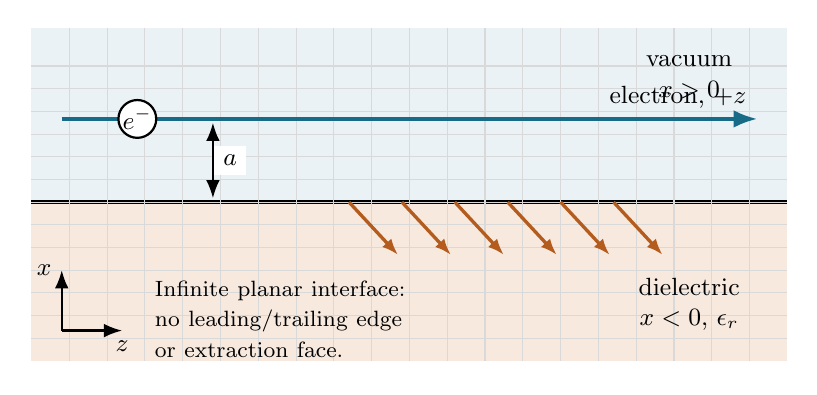
\begin{tikzpicture}[x=0.96cm,y=0.96cm,>=Latex,font=\small]
  \fill[paleblue] (-5,-2.1) rectangle (5,2.3);
  \fill[palebrown] (-5,-2.1) rectangle (5,0);
  \draw[very thick] (-5,0) -- (5,0);
  \foreach \x in {-4.5,-4,-3.5,...,4.5} \draw[gray!30,thin] (\x,-2.1)--(\x,2.3);
  \foreach \y in {-1.8,-1.5,...,2.1} \draw[gray!30,thin] (-5,\y)--(5,\y);
  \draw[very thick,-{Latex[length=3mm]},ipplblue] (-4.6,1.1) -- (4.6,1.1) node[above left,black] {electron, \(+z\)};
  \draw[fill=white,thick] (-3.6,1.1) circle (0.25) node {$e^-$};
  \draw[<->,thick] (-2.6,0.05) -- node[right,fill=white] {$a$} (-2.6,1.05);
  \foreach \x in {-0.8,-0.1,0.6,1.3,2.0,2.7} {
    \draw[very thick,-{Latex[length=2.1mm]},ipplorange] (\x,0) -- ++(0.65,-0.70);
  }
  \node[align=center] at (3.7,1.65) {vacuum\\$x>0$};
  \node[align=center] at (3.7,-1.35) {dielectric\\$x<0$, $\epsilon_r$};
  \draw[->,thick] (-4.6,-1.7) -- (-3.8,-1.7) node[below] {$z$};
  \draw[->,thick] (-4.6,-1.7) -- (-4.6,-0.9) node[left] {$x$};
  \node[align=left,text width=3.2cm] at (-1.7,-1.55) {\footnotesize Infinite planar interface:\\no leading/trailing edge or extraction face.};
\end{tikzpicture}
\vfill
\small \(a\): electron--surface gap; \(x\): surface normal; \(z\): beam axis;
\(y\): direction out of the drawing. Orange arrows show energy entering the dielectric.
\end{frame}

\begin{frame}{A simple ``1-D'' calculation}

The electron follows \((x,y,z)=(a,0,vt)\).
Each Fourier component has phase \(e^{ik_y y+ik_z z-i\omega t}\):
\[
 \omega=2\pi f,\qquad k_z=\frac{\omega}{v}.
\]
Time and \(y\) are Fourier transformed; translation along the trajectory fixes \(k_z\).
For each \((\omega,k_y)\), solve in \(x\):
\[
 \kappa=\sqrt{k_y^2+\frac{\omega^2}{\gamma^2v^2}},
\qquad
 k_{x,d}^{\,2}=\epsilon_r\frac{\omega^2}{c^2}-k_z^2-k_y^2.
\]
\small In vacuum the interface field decays as \(e^{-\kappa a}\).
Real \(k_{x,d}\) allows propagation into the dielectric.

\(k_y\): transverse Fourier wave number. At each radiation frequency, the ``1-D '' code numerically integrates the contributions from the relevant \(k_y\) components.
  %\item \(v=\beta c\): speed; \(c\): vacuum light speed.
  %\item \(\gamma=(1-\beta^2)^{-1/2}=\BeamGamma\): Lorentz factor.
 \(\kappa\): vacuum decay rate; \(k_{x,d}\): normal propagation constant.
 % \item \(\epsilon_r\): real, constant relative permittivity; \(\mu_r=1\): relative permeability.

\source{Planar spectral construction: [1], Sec.~III, Eqs.~(5)--(9); SI convention on the Fourier-normalization slide.}
\end{frame}

\begin{frame}{Single electron: energy flux and energy loss}
Define \(\Ws_1(f)=\dd^2W_1/(\dd z\,\dd f)\):
energy per path length and frequency, in \(\mathrm{J\,m^{-1}\,Hz^{-1}}\).
\[
 \boxed{\Ws_1(f)=-\frac{1}{\pi}\int_{-\infty}^{\infty}\dd k_y\,
  \operatorname{Re}\left[(\widehat\E_d\times\widehat\Hf_d^*)_x\right]}\tag{1}
\]
\small The cross product is spectral Poynting flux.
The minus sign selects energy entering \(x<0\).
Subscript \(d\): dielectric; hats: complex Fourier amplitudes;
\(^*\): complex conjugation; 
\normalsize
\[
 \boxed{\Ws_1(f)=-\frac{q}{\pi}\int_{-\infty}^{\infty}\dd k_y\,
 \operatorname{Re}\widehat E_{z,\mathrm{ref}}(a,k_y,2\pi f)}\tag{2}
\]
\small \(q=-e\): electron charge. The reflected longitudinal field acts back on
the electron; Eq.~(2) measures its energy loss.
\medskip

\textbf{Interpretation:} energy entering the lossless dielectric equals energy
lost by the electron. 
\source{Fields: [1], Sec.~III. Eqs.~(1)--(2) are our SI Poynting/Parseval derivation;
the \(1/\pi\) normalization is explained in the appendix, not copied from [1].}
\end{frame}

\begin{frame}{From the bunch profile to the expected spectrum}
\small The normalized profile \(g(t)\) describes electron arrival times,
with \(\int g(t)\dd t=1\):
\[
 \boxed{F(f)=\int_{-\infty}^{\infty}g(t)e^{i2\pi ft}\dd t
 =\left\langle e^{i2\pi f t_j}\right\rangle}.
\]
\textbf{Meaning:} average the unit waves \(e^{i2\pi ft}\) across the profile \(g(t)\).
\(F\) is the surviving complex amplitude per electron.
\(|F|\simeq1\): waves align; \(|F|\simeq0\): they cancel.

For fixed \(N\), independent arrival times from \(g(t)\), and the same transverse track:
\[
 \boxed{\langle\Ws_N\rangle
 =\underbrace{N\Ws_1}_{\text{individual intensities}}
 +\underbrace{N(N-1)|F|^2\Ws_1}_{\text{interference between electrons}}}\tag{3}
\]
\textbf{What is averaged?} Possible electron arrival times for the
\emph{same} \(N\) and \(g(t)\). No averaging of measured bunches is required.

Eq.~(3) supplies the expected signal and shot-noise reference
from the profile alone. One actual bunch can fluctuate around this prediction.
\source{[2], Eqs.~(29)--(30). The next slide gives the exact spectrum for one specified set of arrival times.}
\end{frame}

\begin{frame}{One actual bunch versus the statistical prediction}
\small If all arrival times \(t_j\) are known, sum their fields directly:
\[
 T_N(f)=\sum_{j=1}^{N}e^{i2\pi f t_j},\qquad
 \boxed{\Ws_N(f)=|T_N(f)|^2\Ws_1(f)}.
\]
\(T_N\) is the \textbf{dimensionless complex phase sum} for one actual bunch.
Each term has magnitude one and phase \(2\pi f t_j\);
\(|T_N|^2\) multiplies the single-electron spectrum, without averaging.
Eq.~(3) is useful when only the smooth profile is specified.

\medskip
%\textbf{Origin of Eq.~(3):}
\(|T_N|^2=N+\sum_{j\ne l}e^{i2\pi f(t_j-t_l)}\).
For independent arrivals, each of the \(N(N-1)\) ordered pairs has expected phase product
\(\langle e^{i2\pi f(t_j-t_l)}\rangle=FF^*=|F|^2\).
\[
 \boxed{\Ws_{\rm fluct}
 =\bigl(\langle|T_N|^2\rangle-|\langle T_N\rangle|^2\bigr)\Ws_1
 =N(1-|F|^2)\Ws_1}\tag{4}
\]
Here \(\langle T_N\rangle=NF\). Eq.~(4) describes field fluctuations about this mean.

For \(F\simeq0\), the smooth mean field cancels,
but the expected intensity remains \(N\Ws_1\): the shot noise.

For the Gaussian envelope used here, \(|F|^2=e^{-(2\pi f\sigma_t)^2}\).
\source{[2], Eqs.~(29)--(30) and Summary, pp.~125--126.
The present Python spectra evaluate Eq.~(3); a specified particle realization uses the direct phase sum.}
\end{frame}

\begin{frame}{Case 1: measuring the full bunch length}
\centering
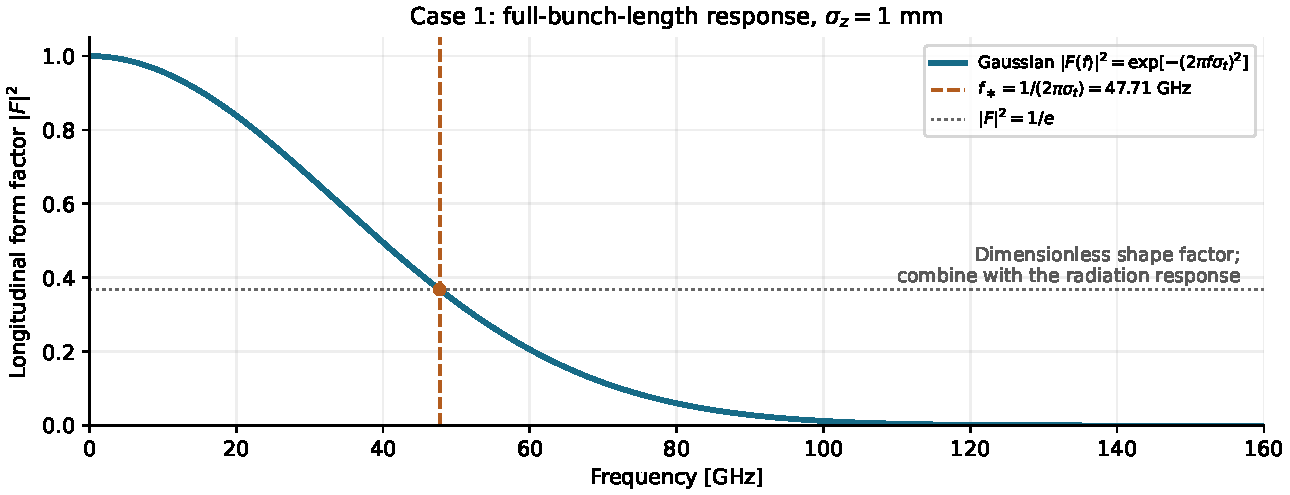
\includegraphics[width=0.86\textwidth]{figures/bunch_length_form_factor.pdf}
\small
\[
 |F(f_*)|^2=e^{-1},\qquad
 f_*=\frac{1}{2\pi\sigma_t}=\FormFactorScaleGHz\ \mathrm{GHz},\qquad
 \sigma_z=\frac{v}{2\pi f_*}.
\]
Fit the coherent spectral roll-off after accounting for the single-electron
response and detector transfer function. Longer wavelengths make this a practical first validation case.
\source{Form-factor diagnostics: [3], Sec.~3, Eqs.~(21), (24)--(27), (33).
The shared-arrival-time argument applies here to ChDR.}
\end{frame}

\begin{frame}{Case 1: coherent signal versus shot noise}
\centering
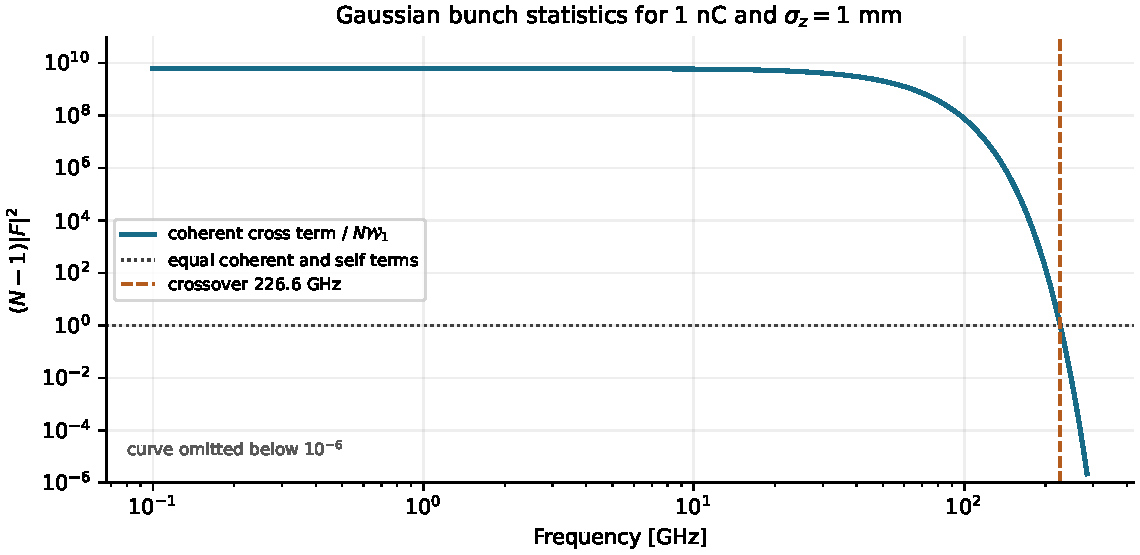
\includegraphics[width=0.88\textwidth]{figures/coherence_crossover.pdf}
\vfill
\small The ratio is \((N-1)|F|^2\), from Eq.~(3).
Interference and individual intensities become equal near \(\CoherenceCrossoverGHz\ \mathrm{GHz}\).
The bunch-length roll-off \(f_*=\FormFactorScaleGHz\ \mathrm{GHz}\) occurs earlier.
\end{frame}

\begin{frame}{Published measurement bands overlap our GHz case}
\begingroup\centering
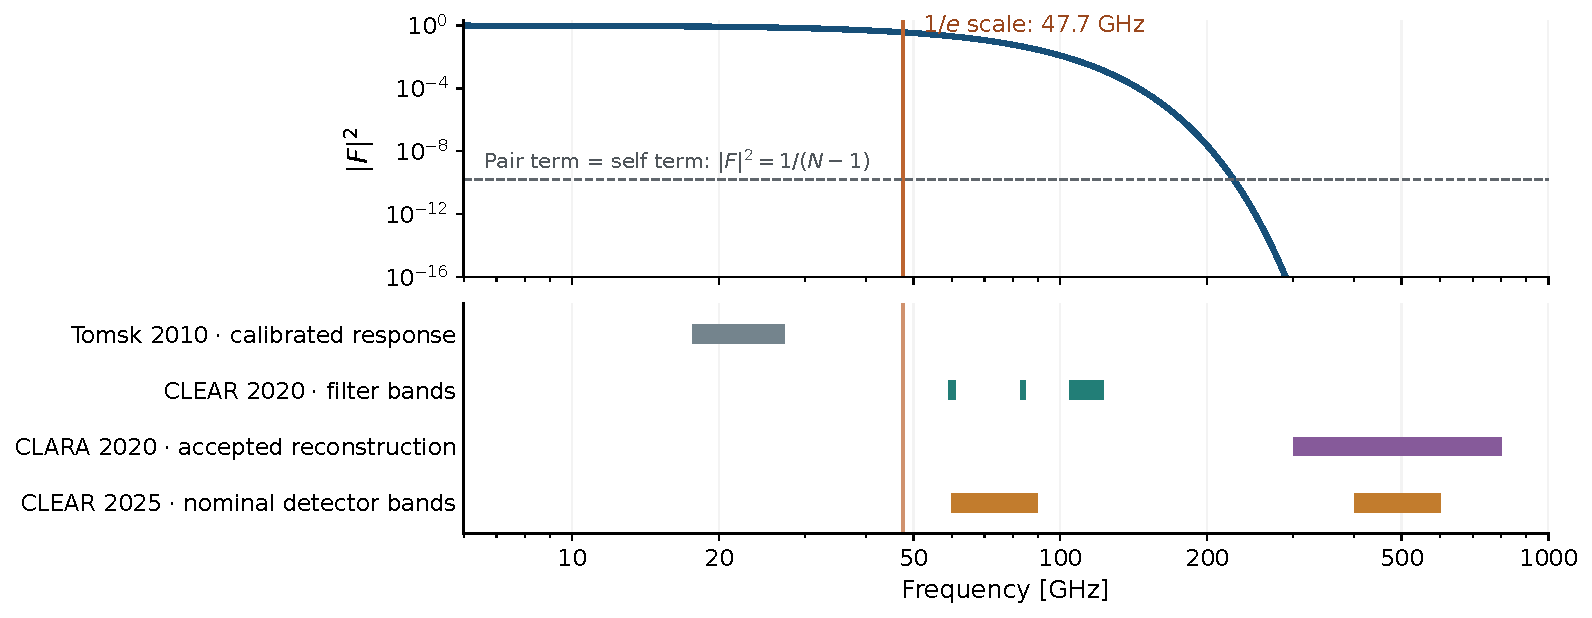
\includegraphics[width=0.94\textwidth]{figures/measurement_bands_vs_bunch.pdf}\par
\endgroup
\smallskip
\small
For our \(1\ \mathrm{mm}\) rms bunch, \textbf{20--120 GHz} spans the spectral slope.
CLEAR's 400--600 GHz channel targets shorter bunches.
\source{Sources: [5]--[7]. Bars indicate detector/filter bands or the accepted reconstruction interval.
The curve contains only the longitudinal form factor. Radiator and detector responses remain to be included.}
\end{frame}

\begin{frame}{Case 2: optical-scale structure within the bunch}
For one bunch, define the \textbf{bunching factor}
\[
 b(f)=\frac{1}{N}\sum_{j=1}^{N}e^{i2\pi f t_j},
 \qquad \boxed{\Ws_N(f)=N^2|b(f)|^2\Ws_1(f)}.
\]
\small \(|b|\) measures phase alignment in that bunch; \(F=\langle b\rangle\)
describes the mean longitudinal profile.
\normalsize
\begin{columns}[T,onlytextwidth]
\column{0.48\textwidth}
\begin{block}{What does \(0.5\ \mu\mathrm{m}\) probe?}
\(\lambda_0=c/f\) is the vacuum wavelength.
A longitudinal modulation at period \(\lambda_b\) gives
\[
 \lambda_b=v/f=\beta\lambda_0.
\]
At 60 MeV, this is approximately \(0.5\ \mu\mathrm{m}\);
the corresponding time period is \(\OpticalPeriodFs\ \mathrm{fs}\).
\end{block}
\column{0.49\textwidth}
\begin{block}{What would indicate microbunching?}
The smooth 1 mm Gaussian has negligible optical \(F\).
Its random bunching level is
\[
 \sqrt{\langle|b|^2\rangle}\simeq N^{-1/2}
 =\ShotNoiseBunchingRms .
\]
An excess or feature above this reference can indicate microstructure,
after calibrating the radiator and detector response.
\end{block}
\end{columns}
\source{Phase summation: [3], Sec.~3.1; random-bunching baseline: [2].
This intrinsic statistical level is not a detector sensitivity limit.}
\end{frame}

\begin{frame}{Case 2: optical shot-noise reference spectrum}
\centering
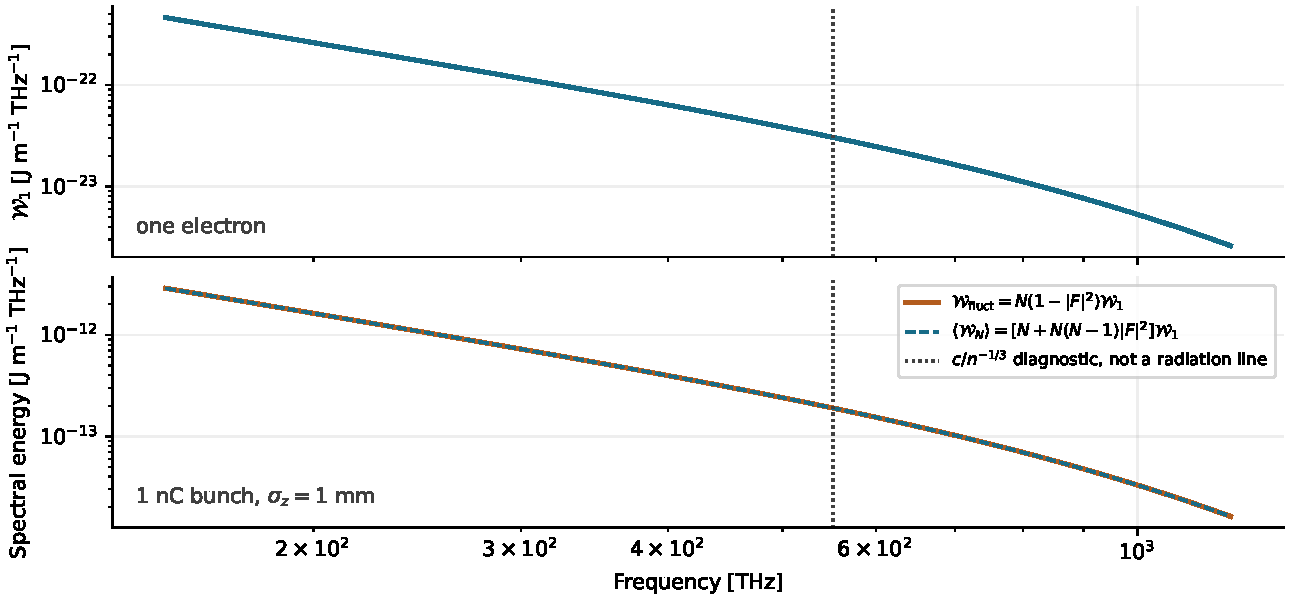
\includegraphics[width=0.84\textwidth]{figures/optical_shot_noise_spectrum.pdf}
\vfill
\scriptsize Smooth Gaussian reference: \(K=\BeamEnergyMeV\ \mathrm{MeV}\), \(Q=1\ \mathrm{nC}\),
\(\sigma_z=1\ \mathrm{mm}\), \(a=10\ \mu\mathrm{m}\), real \(\epsilon_r=2.13\).
At \(\lambda_0=0.5\ \mu\mathrm{m}\), \(\Ws_{\rm fluct}=\OpticalNoise\ \mathrm{J\,m^{-1}\,Hz^{-1}}\).
Compare a future microbunched spectrum with this unmodulated baseline.
\end{frame}

\begin{frame}{Case 2: the gap controls optical coupling}
\begin{columns}[c]
\column{0.64\textwidth}
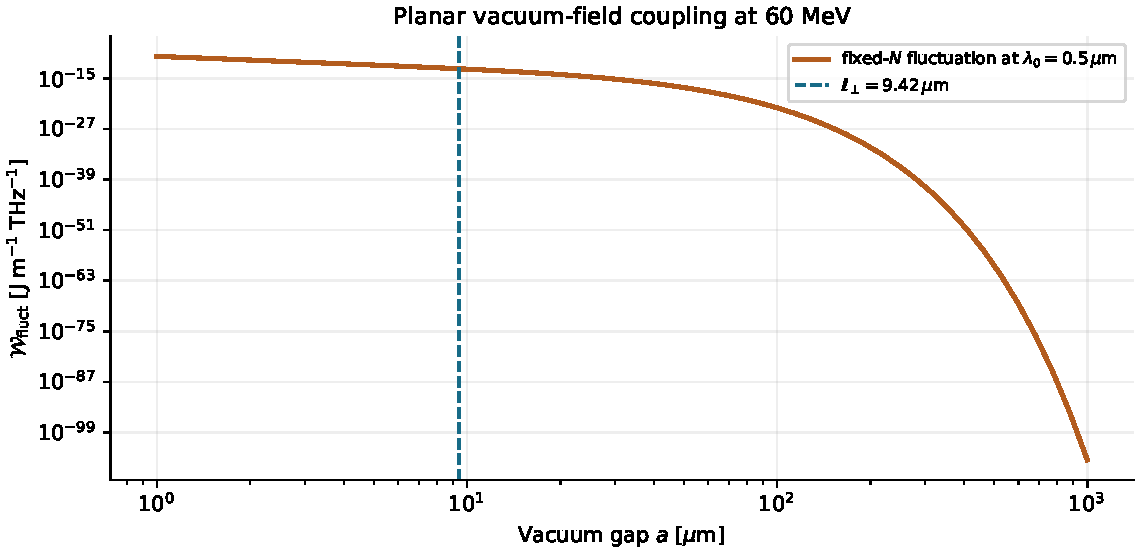
\includegraphics[width=\textwidth]{figures/gap_dependence_0p5um.pdf}
\column{0.33\textwidth}
At \(\lambda_0=0.5\ \mu\mathrm{m}\),
\[
 \ell_\perp=\frac{\gamma\beta\lambda_0}{2\pi}
 =\CouplingLengthUm\ \mu\mathrm{m}.
\]
At the earlier illustrative \(a=1\ \mathrm{mm}\), the least-evanescent exponential coupling factor is
\[
 \exp(-2a/\ell_\perp)=\GapSuppression.
\]
\end{columns}
\vfill
\begin{center}
\small \(\ell_\perp\) is the longest vacuum-field decay length at this frequency.\\
Optical coupling favors electrons close to the surface; use the actual transverse beam distribution to predict the participating charge.
\end{center}
\end{frame}

\begin{frame}{Optical measurements: coupling at 60 MeV}
\small
\begin{tabular}{@{}p{0.21\textwidth}p{0.22\textwidth}p{0.50\textwidth}@{}}
\toprule
\textbf{Experiment} & \textbf{Electrons} & \textbf{Optical selection}\\
\midrule
CESR [8] & 5.3 GeV & \(600\pm10\) nm as reported in figure captions\\[0.5em]
ATF2 [9] & 1.3 GeV & 700 nm centre, nominal 40 nm FWHM filter\\[0.5em]
CLEAR [10] & 200 MeV & \(600\pm10\) nm, preliminary in-air result\\
\bottomrule
\end{tabular}
\medskip

These experiments establish incoherent optical ChDR for beam imaging or position.
The reviewed sources contain no demonstration of optical ChDR microbunching diagnostics.
\[
\ell_\perp=\frac{\gamma\beta\lambda_0}{2\pi}
=\CouplingLengthUm\ \mu\mathrm{m}
\qquad (60\ \mathrm{MeV},\ \lambda_0=0.5\ \mu\mathrm{m}).
\]
\textbf{Our design constraint:} a \(10\ \mu\mathrm{m}\) centre gap would intercept
a substantial part of a \(1\ \mathrm{mm}\) rms beam.
Optical coupling needs a consistent normal beam size and clearance.
\source{[8] Secs.~III--IV; [9] p.~2656 and filter specification; [10] pp.~662--663.
CESR prose calls the filter ``10 nm bandpass'', so its FWHM remains ambiguous.
CLEAR's large-gap in-air signal needs separate assessment against our vacuum model.}
\end{frame}

\begin{frame}{What this model can validate in IPPL}
\begin{columns}[T]
\column{0.48\textwidth}
\begin{block}{Direct comparisons}
\begin{itemize}
  \item complex fields at specified laboratory probes;
  \item TE/TM interface behavior and dielectric propagation angle;
  \item gap dependence and flux/work energy consistency;
  \item the single-electron spectral response before bunch statistics.
\end{itemize}
\end{block}
\column{0.48\textwidth}
\begin{block}{Route from reference to experiment}
\begin{itemize}
  \item include the finite prism and its optical extraction face;
  \item use measured, frequency-dependent complex \(\epsilon(\omega)\);
  \item include transverse beam size and the distribution of gaps;
  \item calibrate detector bandwidth and collection optics.
\end{itemize}
\end{block}
\end{columns}
\vfill
\begin{block}{Recommended sequence}
Case 1: validate the coherent bunch-length signal.
Case 2: add prescribed microbunching and compare its spectrum with the noise reference.
\end{block}
\source{Moving sources in FDTD: [4], Sec.~4.7.
Numerical checks use common field phases, spectral normalization and geometry.}
\end{frame}

\begin{frame}{Appendix: Fourier convention and the \(1/\pi\) factor}
\small For the electric field \(\mathbf U=\E\) or magnetic field strength \(\mathbf U=\Hf\), we use
\[
 \mathbf U(x,y,z,t)=\frac{1}{(2\pi)^2}
 \int\dd\omega\,\dd k_y\,
 \widehat{\mathbf U}(x,k_y,\omega)
 e^{ik_y y+i\omega z/v-i\omega t}.
\]
The transformed charge and current densities are
\(\widehat\rho=(q/v)\delta(x-a)\) and \(\widehat J_z=q\delta(x-a)\).
The Dirac delta \(\delta\) locates the electron at \(x=a\).
\[
 \frac{W_1}{L}
 =-\int\dd t\,\dd y\,(\E_d\times\Hf_d)_x
 =-\frac{1}{(2\pi)^2}
 \int\dd\omega\,\dd k_y\,
 \operatorname{Re}(\widehat\E_d\times\widehat\Hf_d^*)_x .
\]
Parseval's identity converts time/position integration to a product of Fourier amplitudes.
Real fields give equal contributions at positive and negative frequency.
With \(\dd\omega=2\pi\,\dd f\),
\[
 \underbrace{\frac{2(2\pi)}{(2\pi)^2}}_{f>0}=\frac{1}{\pi}.
\]
Here \(L\) is trajectory length; \(\widehat\E\) has units \(\mathrm{V\,s}\),
\(\widehat\Hf\) has units \(\mathrm{A\,s}\).
\source{Local SI derivation of Eq.~(1). Applying the same inverse transform to
the induced work \(-qE_{z,\mathrm{ref}}\) gives Eq.~(2). Field construction: [1].}
\end{frame}

\begin{frame}{Reproducibility and references}
\textbf{In this directory}
\begin{itemize}
  \item \texttt{make\_figures.py}: regenerates the figures from \texttt{../chdr\_1d.py};
  \item \texttt{chdr\_1d\_presentation.tex}: TeXShop-ready Beamer source;
  \item \texttt{Makefile}: \texttt{make figures} then \texttt{make pdf}.
\end{itemize}
\vspace{0.4em}
\textbf{References}
\begin{enumerate}\footnotesize
  \item A.~V.~Tyukhtin, S.~N.~Galyamin and V.~V.~Vorobev,
  \emph{Radiation of Charge Moving along Face of Inverted Prism},
  \href{https://arxiv.org/abs/2105.01111}{arXiv:2105.01111v2} (2022).
  Sec.~III, Eqs.~(5)--(9): planar field construction (Gaussian units).
  \item R.~A.~Bosch and R.~J.~Bosch,
  \emph{Derivation of Bunching for Poisson Statistics},
  \href{https://proceedings.jacow.org/FEL2009/papers/mopc44.pdf}{FEL2009, MOPC44, pp.~123--126}.
  Eqs.~(29)--(30) and p.~126: moments at \emph{fixed} electron count.
  \item B.~Schmidt et al.,
  \emph{Longitudinal Bunch Diagnostics using Coherent Transition Radiation Spectroscopy},
  \href{https://arxiv.org/abs/1803.00608}{DESY 18-027 (2018)}.
  Sec.~3, Eqs.~(21), (24)--(27), (33): phase summation and form factors.
  \item A.~Oskooi and S.~G.~Johnson,
  \emph{Electromagnetic Wave Source Conditions}, in
  \emph{Advances in FDTD Computational Electrodynamics}, eds.
  A.~Taflove, A.~Oskooi and S.~G.~Johnson (2013).
  \href{https://arxiv.org/abs/1301.5366}{Chapter 4}, Sec.~4.7: moving charges.
\end{enumerate}
\end{frame}

\begin{frame}{Measurement literature}
\begin{enumerate}\footnotesize
\setcounter{enumi}{4}
  \item A.~P.~Potylitsyn et al., \emph{Coherent Cherenkov Radiation from a Short
  Bunch Passing near a Target and Possibility of a Bunch Length Diagnostics},
  \href{https://accelconf.web.cern.ch/IPAC10/papers/mope046.pdf}{IPAC2010, MOPE046}.
  Experimental section: calibrated detector band and \(\sigma_z=1.2\) mm.
  \item A.~Curcio et al., \emph{Noninvasive bunch length measurements exploiting
  Cherenkov diffraction radiation},
  \href{https://doi.org/10.1103/PhysRevAccelBeams.23.022802}{PRAB \textbf{23}, 022802 (2020)}.
  Secs.~IV--V: CLEAR channels and CLARA spectral reconstruction.
  \item C.~Davut et al., \emph{Design and experimental verification of a bunch
  length monitor based on coherent Cherenkov diffraction radiation},
  \href{https://doi.org/10.1103/PhysRevResearch.7.013193}{PRResearch \textbf{7}, 013193 (2025)}.
  Tables~II--III and Sec.~V: detector bands and measured beam parameters.
  \item R.~Kieffer et al., \emph{Generation of incoherent Cherenkov diffraction
  radiation in synchrotrons},
  \href{https://doi.org/10.1103/PhysRevAccelBeams.23.042803}{PRAB \textbf{23}, 042803 (2020)}.
  \item M.~Bergamaschi et al., \emph{Recent Results using Incoherent Cherenkov
  Diffraction Radiation for Non-Invasive Beam Diagnostics},
  \href{https://proceedings.jacow.org/ipac2019/papers/wepgw077.pdf}{IPAC2019, WEPGW077}.
  \href{https://www.thorlabs.com/catalogpages/V21/395.pdf}{Thorlabs FB700-40 specification}, p.~395.
  \item D.~Alves et al., \emph{Cherenkov Diffraction Radiation as a Tool for Beam
  Diagnostics},
  \href{https://proceedings.jacow.org/ibic2019/papers/thao01.pdf}{IBIC2019, THAO01}.
\end{enumerate}
\vfill
\scriptsize Band comparison generator: \texttt{../../ideas-lit-reseach/compare\_measurement\_bands.py}.
\texttt{make figures} regenerates the comparison and copies its slide version here.
\end{frame}

\end{document}
